\documentclass[a4paper,14pt,oneside,final]{extarticle}
\usepackage[top=2cm, bottom=2cm, left=3cm, right=1cm]{geometry}
\usepackage{scrextend}

\usepackage[T2A,T1]{fontenc}
\usepackage[ukrainian,russian,english]{babel}
\usepackage{tempora}
\usepackage{fontspec}
\setmainfont{tempora}

% Зачем: Отключает использование изменяемых межсловных пробелов.
% Почему: Так не принято делать в текстах на русском языке.
\frenchspacing

\usepackage{indentfirst}
\setlength{\parindent}{1.25cm}
\renewcommand{\baselinestretch}{1.5}

% Header
\usepackage{fancyhdr}
\pagestyle{fancy}
\fancyhead{}
\fancyfoot{}
\fancyhead[R]{\small \selectfont \thepage}
\renewcommand{\headrulewidth}{0pt}

% Captions
\usepackage{chngcntr}
\counterwithin{figure}{section}
\counterwithin{table}{section}
\usepackage[tableposition=top]{caption}
\usepackage{subcaption}
\DeclareCaptionLabelFormat{gostfigure}{Рисунок #2}
\DeclareCaptionLabelFormat{gosttable}{Таблиця #2}
\DeclareCaptionLabelSeparator{gost}{~---~}
\captionsetup{labelsep=gost}
\captionsetup[figure]{labelformat=gostfigure}
\captionsetup[table]{labelformat=gosttable}
\renewcommand{\thesubfigure}{\asbuk{subfigure}}

% Sections
\usepackage[explicit]{titlesec}
\newcommand{\sectionbreak}{\clearpage}

\titleformat{\section}
  {\centering}{\thesection \quad}{0pt}{\MakeUppercase{#1}}
\titleformat{\subsection}[block]
  {\bfseries}{\thesubsection \quad #1}{0cm}{}

\titlespacing{\section} {0cm}{0cm}{21pt}
\titlespacing{\subsection} {\parindent}{21pt}{0cm}
\titlespacing{\subsubsection} {\parindent}{0cm}{0cm}

% Lists
\usepackage{enumitem}
\renewcommand\labelitemi{--}
\setlist[itemize]{noitemsep, topsep=0pt, wide}
\setlist[enumerate]{noitemsep, topsep=0pt, wide, label=\arabic*}
\setlist[description]{labelsep=0pt, noitemsep, topsep=0pt, leftmargin=2\parindent, labelindent=\parindent, labelwidth=\parindent, font=\normalfont}

% Toc
\usepackage{tocloft}
\tocloftpagestyle{fancy}
\renewcommand{\cfttoctitlefont}{}
\setlength{\cftbeforesecskip}{0pt}
\renewcommand{\cftsecfont}{}
\renewcommand{\cftsecpagefont}{}
\renewcommand{\cftsecleader}{\cftdotfill{\cftdotsep}}

\usepackage{float}
\usepackage{pgfplots}
\usepackage{graphicx}
\usepackage{multirow}
\usepackage{amssymb,amsfonts,amsmath,amsthm}
\usepackage{csquotes}

\usepackage{listings}
\lstset{basicstyle=\footnotesize\ttfamily,breaklines=true}
\lstset{language=Matlab}

\usepackage[
	backend=biber,
	sorting=none,
	language=auto,
	autolang=other
]{biblatex}
\DeclareFieldFormat{labelnumberwidth}{#1}

\lstdefinelanguage{Python}{
  keywords={and, break, class, continue, def, yield, del, elif, else, except, exec, finally, for, from, global, if, import, in, lambda, not, or, pass, print, raise, return, try, while, assert, with},
  keywordstyle=\color{NavyBlue}\bfseries,
  ndkeywords={True, False},
  ndkeywordstyle=\color{BurntOrange}\bfseries,
  emph={as},
  emphstyle={\color{OrangeRed}},
  identifierstyle=\color{black},
  sensitive=true,
  commentstyle=\color{gray}\ttfamily,
  comment=[l]{\#},
  morecomment=[s]{/*}{*/},
  stringstyle=\color{ForestGreen}\ttfamily,
  morestring=[b]',
  morestring=[s]{"""*}{*"""},
}


\newcommand{\labnumber}{2} % second lab
\documentclass[a4paper,14pt,oneside,final]{extarticle}
\usepackage[top=2cm, bottom=2cm, left=3cm, right=1cm]{geometry}
\usepackage{scrextend}

\usepackage[T2A,T1]{fontenc}
\usepackage[ukrainian,russian,english]{babel}
\usepackage{tempora}
\usepackage{fontspec}
\setmainfont{tempora}

% Зачем: Отключает использование изменяемых межсловных пробелов.
% Почему: Так не принято делать в текстах на русском языке.
\frenchspacing

\usepackage{indentfirst}
\setlength{\parindent}{1.25cm}
\renewcommand{\baselinestretch}{1.5}

% Header
\usepackage{fancyhdr}
\pagestyle{fancy}
\fancyhead{}
\fancyfoot{}
\fancyhead[R]{\small \selectfont \thepage}
\renewcommand{\headrulewidth}{0pt}

% Captions
\usepackage{chngcntr}
\counterwithin{figure}{section}
\counterwithin{table}{section}
\usepackage[tableposition=top]{caption}
\usepackage{subcaption}
\DeclareCaptionLabelFormat{gostfigure}{Рисунок #2}
\DeclareCaptionLabelFormat{gosttable}{Таблиця #2}
\DeclareCaptionLabelSeparator{gost}{~---~}
\captionsetup{labelsep=gost}
\captionsetup[figure]{labelformat=gostfigure}
\captionsetup[table]{labelformat=gosttable}
\renewcommand{\thesubfigure}{\asbuk{subfigure}}

% Sections
\usepackage[explicit]{titlesec}
\newcommand{\sectionbreak}{\clearpage}

\titleformat{\section}
  {\centering}{\thesection \quad}{0pt}{\MakeUppercase{#1}}
\titleformat{\subsection}[block]
  {\bfseries}{\thesubsection \quad #1}{0cm}{}

\titlespacing{\section} {0cm}{0cm}{21pt}
\titlespacing{\subsection} {\parindent}{21pt}{0cm}
\titlespacing{\subsubsection} {\parindent}{0cm}{0cm}

% Lists
\usepackage{enumitem}
\renewcommand\labelitemi{--}
\setlist[itemize]{noitemsep, topsep=0pt, wide}
\setlist[enumerate]{noitemsep, topsep=0pt, wide, label=\arabic*}
\setlist[description]{labelsep=0pt, noitemsep, topsep=0pt, leftmargin=2\parindent, labelindent=\parindent, labelwidth=\parindent, font=\normalfont}

% Toc
\usepackage{tocloft}
\tocloftpagestyle{fancy}
\renewcommand{\cfttoctitlefont}{}
\setlength{\cftbeforesecskip}{0pt}
\renewcommand{\cftsecfont}{}
\renewcommand{\cftsecpagefont}{}
\renewcommand{\cftsecleader}{\cftdotfill{\cftdotsep}}

\newcommand{\khpistudentgroup}{КН-34г}
\newcommand{\khpistudentname}{Чепурний~А.~С.}

\newcommand{\khpidepartment}{Програмна інженерія та інформаційні технології управління}
\newcommand{\khpititlewhat}{
	Лабораторна робота №\labnumber \\
	з предмету <<Моделювання систем>>
}
\newcommand{\khpititlewho}{
	Виконав: \\
	\hspace*{\parindent} ст. групи \khpistudentgroup \\
	\hspace*{\parindent} \khpistudentname \\
	Перевірила: \\
	\hspace*{\parindent} ст. в. каф. ПІІТУ \\
	\hspace*{\parindent} Єршова~С.~І. \\
	\hspace*{\parindent} ас. каф. ПІІТУ \\
	\hspace*{\parindent} Литвинова~Ю.~С. \\
}



\graphicspath{{figures/}}

\begin{document}
\Russian

\begin{titlepage}

\begin{center}
	МІНІСТЕРСТВО ОСВІТИ І НАУКИ УКРАЇНИ \\
	НАЦІОНАЛЬНИЙ ТЕХНІЧНИЙ УНІВЕРСИТЕТ \\
	«ХАРКІВСЬКИЙ ПОЛІТЕХНІЧНИЙ ІНСТИТУТ» \\[0.5cm]
	Кафедра <<\khpidepartment>> \\
\end{center}

\vspace{6cm}

\begin{center}
	\khpititlewhat
\end{center}

\vspace{3cm}

\begin{addmargin}[10cm]{0cm}
	\khpititlewho
\end{addmargin}

\vspace{\fill}

\begin{center}
	Харків \the\year
\end{center}

\end{titlepage}

\addtocounter{page}{1}

\section*{Программирование нейронных сетей}
\subsubsection*{Цель работы}
Получить практические навыки программирования нейронных сетей на языке Python.
\subsubsection*{Постановка задачи}
Необходимо с помощью одно- и многослоевой нейронной сети симулировать функцию $\sin x$.

\subsection*{Общая нейронная сеть}
Класс \texttt{Network} предоставляет возможность создавать нейронные сети разной структуры и обучать их методом обратного распространения ошибки: 
\lstinputlisting{code/network.py} 

Класс \texttt{Experiment} позволяет создавать нейронные сети разных структур и проводить над ними эксперимет по моделированию функции $\sin x$:
\lstinputlisting{code/experiment.py} 


\subsection*{Однослойная нейронная сеть}
Исходный код эксперимента:  
\lstinputlisting{code/task_single_layer.py} 

Результат работы представлен на рисунке~\ref{fig:single_layer_result}.

\begin{figure}[H]
    \centering
        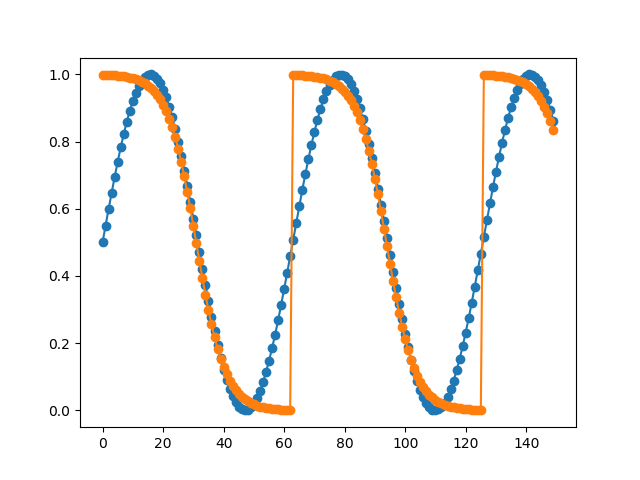
\includegraphics[width=0.7\textwidth]{single_layer_result}
    \caption{Результат прогнозирования функции $\sin x$ однослойной сетью}
    \label{fig:single_layer_result}
\end{figure}

\subsection{Многослойная нейронная сеть}
Исходный код эксперимента:  
\lstinputlisting{code/task_multi_layer.py} 

Результат работы представлен на рисунке~\ref{fig:multi_layer_result}.

\begin{figure}[H]
    \centering
        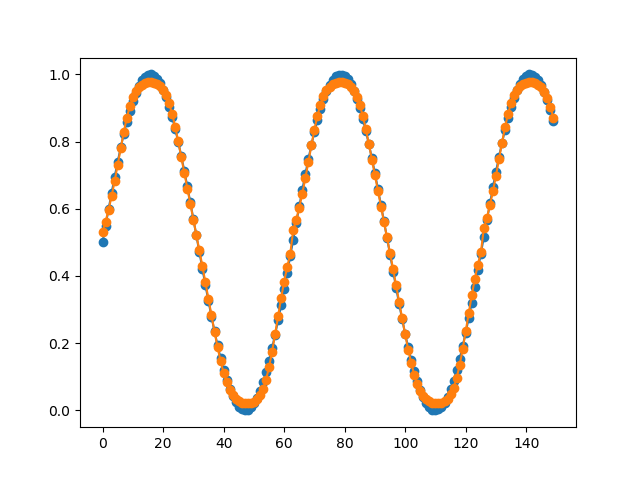
\includegraphics[width=0.7\textwidth]{multi_layer_result}
    \caption{Результат прогнозирования функции $\sin x$ многослойной сетью}
    \label{fig:multi_layer_result}
\end{figure}

\subsection*{Выводы}
В результате выполнения данной лабораторной работы были получены практические навыки программирования нейронных сетей на языке Python.

Однослойная нейронная сеть способна только к линейной квалификации, в отличии от многослойной.

\end{document}
